\documentclass[svgnames,11pt]{beamer}
\input{/home/tof/Documents/Cozy/latex-include/preambule_commun.tex}
\input{/home/tof/Documents/Cozy/latex-include/preambule_beamer.tex}
%\usepackage{pgfpages} \setbeameroption{show notes on second screen=left}
\author[]{Christophe Viroulaud}
\title{Détection de cycle dans un graphe orienté}
\date{\framebox{\textbf{Algo 19}}}
%\logo{}
\institute{Terminale - NSI}

\begin{document}
\begin{frame}
    \titlepage
\end{frame}
\begin{frame}
    \frametitle{}

    \begin{itemize}
        \item<1-> La réalisation d'un projet est découpée en plusieurs tâches.
        \item<2-> Certaines tâches doivent être réalisées avant d'autres.
    \end{itemize}

\end{frame}
\begin{frame}
    \frametitle{}

    \underline{Projet: }Construire une maison
    \begin{enumerate}
        \item Construire les fondations.
        \item Construire les murs.
        \item Poser la toiture.
        \item Monter les cloisons.
        \item \dots
    \end{enumerate}

\end{frame}
\begin{frame}
    \frametitle{}


    \begin{center}
        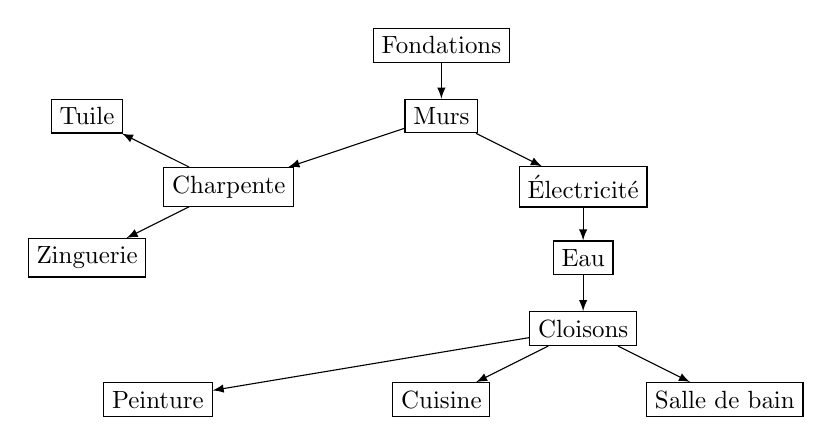
\begin{tikzpicture}[scale=0.9,transform shape]
            \node[draw] (A)at(0,0) {Fondations};
            \node[draw] (B)at(0,-1) {Murs};
            \node[draw] (B1)at(2,-2) {Électricité};
            \node[draw] (B2)at(2,-3) {Eau};

            \node[draw] (C)at(-3,-2) {Charpente};
            \node[draw] (C1)at(-5,-1) {Tuile};
            \node[draw] (C2)at(-5,-3) {Zinguerie};
            \node[draw] (D)at(2,-4) {Cloisons};
            \node[draw] (E)at(-4,-5) {Peinture};
            \node[draw] (F)at(0,-5) {Cuisine};
            \node[draw] (G)at(4,-5) {Salle de bain};


            \draw[->,>=latex] (A) -- (B);
            \draw[->,>=latex] (B) -- (B1);
            \draw[->,>=latex] (B1) -- (B2);
            \draw[->,>=latex] (B2) -- (D);
            \draw[->,>=latex] (B) -- (C);
            \draw[->,>=latex] (D) -- (E);
            \draw[->,>=latex] (D) -- (F);
            \draw[->,>=latex] (D) -- (G);
            \draw[->,>=latex] (C) -- (C1);
            \draw[->,>=latex] (C) -- (C2);

        \end{tikzpicture}
        \captionof{figure}{\centering On représente l'ordonnancement des tâches par un graphe de précédences.}
    \end{center}

\end{frame}
\begin{frame}
    \frametitle{}

    On représente l'ordonnancement des tâches par un graphe de précédences.
    \begin{center}
        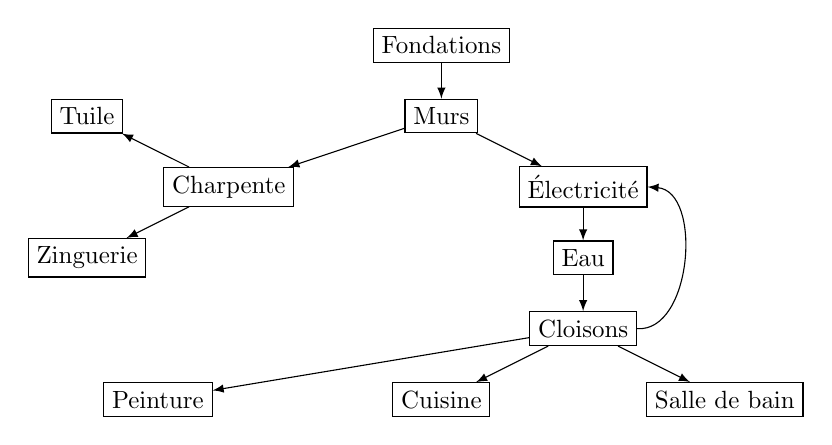
\begin{tikzpicture}[scale=0.9,transform shape]
            \node[draw] (A)at(0,0) {Fondations};
            \node[draw] (B)at(0,-1) {Murs};
            \node[draw] (B1)at(2,-2) {Électricité};
            \node[draw] (B2)at(2,-3) {Eau};

            \node[draw] (C)at(-3,-2) {Charpente};
            \node[draw] (C1)at(-5,-1) {Tuile};
            \node[draw] (C2)at(-5,-3) {Zinguerie};
            \node[draw] (D)at(2,-4) {Cloisons};
            \node[draw] (E)at(-4,-5) {Peinture};
            \node[draw] (F)at(0,-5) {Cuisine};
            \node[draw] (G)at(4,-5) {Salle de bain};


            \draw[->,>=latex] (A) -- (B);
            \draw[->,>=latex] (B) -- (B1);
            \draw[->,>=latex] (B1) -- (B2);
            \draw[->,>=latex] (B2) -- (D);
            \draw[->,>=latex] (B) -- (C);
            \draw[->,>=latex] (D) -- (E);
            \draw[->,>=latex] (D) -- (F);
            \draw[->,>=latex] (D) -- (G);
            \draw[->,>=latex] (C) -- (C1);
            \draw[->,>=latex] (C) -- (C2);
            \draw[->,>=latex] (D.east) to[bend right=90] (B1.east);

        \end{tikzpicture}
        \captionof{figure}{Problème dans l'ordonnancement}
    \end{center}

\end{frame}
\begin{frame}
    \frametitle{}

    \begin{framed}
        \centering Comment repérer un cycle dans un graphe orienté?
    \end{framed}

\end{frame}
\section{Définition}
\subsection{Cycle dans un graphe}
\begin{frame}
    \frametitle{Définition - cycle dans un graphe}

    \begin{aretenir}[]
        Dans un graphe, un \textbf{cycle} est un \textbf{chemin} qui part d'un sommet et revient à ce même sommet.
    \end{aretenir}

\end{frame}
\subsection{Vocabulaire}

\begin{frame}
    \frametitle{Vocabulaire}

    \begin{center}
        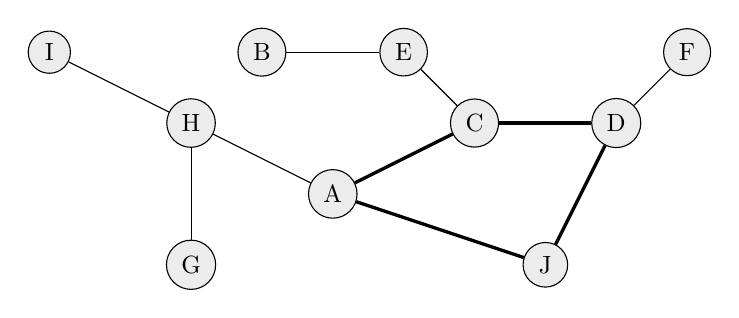
\begin{tikzpicture}[scale=0.9,transform shape]
            \node[draw,circle,fill=gray!15] (A)at(0,0) {A};
            \node[draw,circle,fill=gray!15] (B)at(-1,2) {B};
            \node[draw,circle,fill=gray!15] (C)at(2,1) {C};
            \node[draw,circle,fill=gray!15] (D)at(4,1) {D};
            \node[draw,circle,fill=gray!15] (E)at(1,2) {E};
            \node[draw,circle,fill=gray!15] (F)at(5,2) {F};
            \node[draw,circle,fill=gray!15] (G)at(-2,-1) {G};
            \node[draw,circle,fill=gray!15] (H)at(-2,1) {H};
            \node[draw,circle,fill=gray!15] (I)at(-4,2) {I};
            \node[draw,circle,fill=gray!15] (J)at(3,-1) {J};
            \draw[-,>=latex] (E) -- (B);
            \draw[-,>=latex, very thick] (A) -- (C);
            \draw[-,>=latex] (A) -- (H);
            \draw[-,>=latex, very thick] (A) -- (J);
            \draw[-,>=latex] (H) -- (I);
            \draw[-,>=latex] (H) -- (G);
            \draw[-,>=latex] (C) -- (E);
            \draw[-,>=latex, very thick] (C) -- (D);
            %\draw[-,>=latex] (C) -- (J);
            \draw[-,>=latex, very thick] (D) -- (J);
            \draw[-,>=latex] (D) -- (F);

        \end{tikzpicture}
        \captionof{figure}{\centering \textbf{Chaîne} et \textbf{cycle} dans un graphe non orienté}
    \end{center}
    \begin{itemize}
        \item une \textbf{chaîne:} I - H - A
        \item un \textbf{cycle:} A - J - D - C
    \end{itemize}
\end{frame}
\begin{frame}
    \frametitle{}

    \begin{center}
        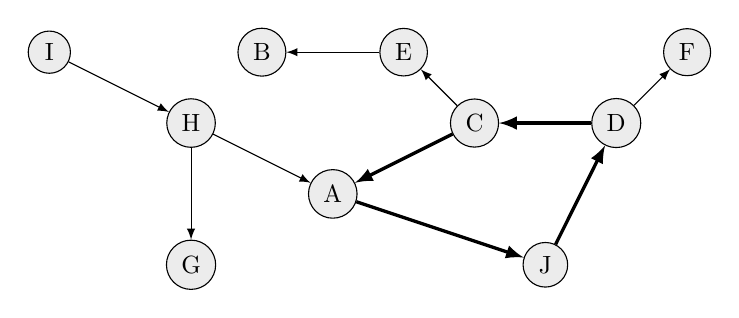
\begin{tikzpicture}[scale=0.9,transform shape]
            \node[draw,circle,fill=gray!15] (A)at(0,0) {A};
            \node[draw,circle,fill=gray!15] (B)at(-1,2) {B};
            \node[draw,circle,fill=gray!15] (C)at(2,1) {C};
            \node[draw,circle,fill=gray!15] (D)at(4,1) {D};
            \node[draw,circle,fill=gray!15] (E)at(1,2) {E};
            \node[draw,circle,fill=gray!15] (F)at(5,2) {F};
            \node[draw,circle,fill=gray!15] (G)at(-2,-1) {G};
            \node[draw,circle,fill=gray!15] (H)at(-2,1) {H};
            \node[draw,circle,fill=gray!15] (I)at(-4,2) {I};
            \node[draw,circle,fill=gray!15] (J)at(3,-1) {J};
            \draw[->,>=latex] (E) -- (B);
            \draw[<-,>=latex, very thick] (A) -- (C);
            \draw[<-,>=latex] (A) -- (H);
            \draw[->,>=latex, very thick] (A) -- (J);
            \draw[<-,>=latex] (H) -- (I);
            \draw[->,>=latex] (H) -- (G);
            \draw[->,>=latex] (C) -- (E);
            \draw[<-,>=latex, very thick] (C) -- (D);
            %\draw[-,>=latex] (C) -- (J);
            \draw[<-,>=latex, very thick] (D) -- (J);
            \draw[->,>=latex] (D) -- (F);

        \end{tikzpicture}
        \captionof{figure}{\centering \textbf{Chemin} et \textbf{circuit} dans un graphe orienté}
    \end{center}
    \begin{itemize}
        \item un \textbf{chemin:} I - H - A
        \item un \textbf{circuit:} A - J - D - C
    \end{itemize}
\end{frame}
\begin{frame}
    \frametitle{}

    \begin{aretenir}[Remarque]
        Dans de nombreux ouvrages, les termes \textbf{cycle} et \textbf{circuit}  ainsi que \textbf{chaîne} et \textbf{chemin}, sont indifférenciés.
    \end{aretenir}

\end{frame}
\subsection{Cas de figures}
\begin{frame}
    \frametitle{Cas de figures}

    \begin{multicols}{2}
        \begin{center}
            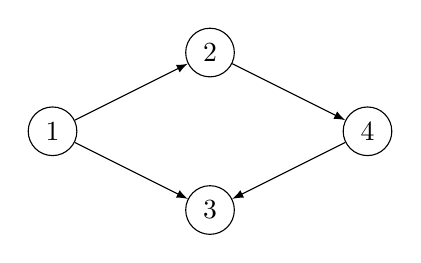
\begin{tikzpicture}
                \node[draw,circle] (A)at(0,0) {1};
                \node[draw,circle] (B)at(2,1) {2};
                \node[draw,circle] (C)at(2,-1) {3};
                \node[draw,circle] (D)at(4,0) {4};


                \draw[->,>=latex] (A) -- (B);
                \draw[->,>=latex] (A) -- (C);
                \draw[->,>=latex] (B) -- (D);
                \draw[<-,>=latex] (C) -- (D);
            \end{tikzpicture}
            \captionof{figure}{Pas de circuit}
        \end{center}

        \begin{center}
            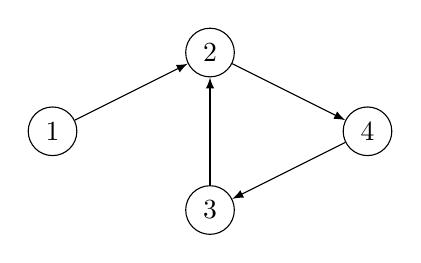
\begin{tikzpicture}
                \node[draw,circle] (A)at(0,0) {1};
                \node[draw,circle] (B)at(2,1) {2};
                \node[draw,circle] (C)at(2,-1) {3};
                \node[draw,circle] (D)at(4,0) {4};
                \draw[->,>=latex] (A) -- (B);
                \draw[<-,>=latex] (B) -- (C);
                \draw[->,>=latex] (B) -- (D);
                \draw[<-,>=latex] (C) -- (D);
            \end{tikzpicture}
            \captionof{figure}{Circuit}
        \end{center}
    \end{multicols}
    \begin{aretenir}[Observation]
        Dans ces graphes, un parcours en profondeur partant de A affiche 1 - 2 - 4 - 3, mais ne détecte pas le cycle.
    \end{aretenir}
\end{frame}
\section{Détection de cycle}
\subsection{Modification du parcours en profondeur}
\begin{frame}
    \frametitle{Détection de cycle - Modification du DFS}

    On distingue trois états pour les sommets:
    \begin{itemize}
        \item \textbf{BLANC:} sommet non encore atteint,
        \item \textbf{GRIS:} sommet en cours de visite,
        \item \textbf{NOIR:} sommet dont le parcours est terminé.
    \end{itemize}

\end{frame}
\begin{frame}
    \frametitle{}

    \begin{aretenir}[]
        \begin{itemize}
            \item On note en \textbf{GRIS} les sommets pour lesquels on n'a pas encore visités tous les voisins.
            \item On note en \textbf{NOIR} les sommets pour lesquels tous les voisins ont été visités.
        \end{itemize}
    \end{aretenir}

\end{frame}

\begin{frame}
    \frametitle{}

    \begin{center}
        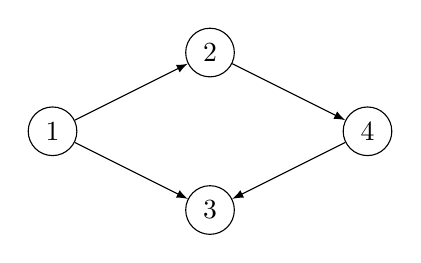
\begin{tikzpicture}
            \node[draw,circle] (A)at(0,0) {1};
            \node[draw,circle] (B)at(2,1) {2};
            \node[draw,circle] (C)at(2,-1) {3};
            \node[draw,circle] (D)at(4,0) {4};


            \draw[->,>=latex] (A) -- (B);
            \draw[->,>=latex] (A) -- (C);
            \draw[->,>=latex] (B) -- (D);
            \draw[<-,>=latex] (C) -- (D);
        \end{tikzpicture}
        \captionof{figure}{\centering Initialisation: tous les sommets en \textbf{\texttt{BLANC}}}
    \end{center}

\end{frame}
\begin{frame}
    \frametitle{}

    \begin{center}
        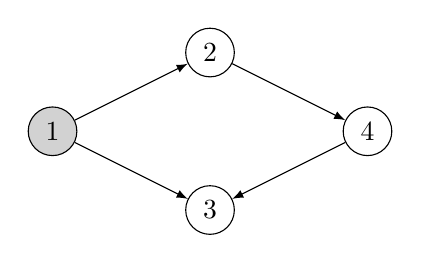
\begin{tikzpicture}
            \node[draw,circle,fill=gray!35] (A)at(0,0) {1};
            \node[draw,circle] (B)at(2,1) {2};
            \node[draw,circle] (C)at(2,-1) {3};
            \node[draw,circle] (D)at(4,0) {4};


            \draw[->,>=latex] (A) -- (B);
            \draw[->,>=latex] (A) -- (C);
            \draw[->,>=latex] (B) -- (D);
            \draw[<-,>=latex] (C) -- (D);
        \end{tikzpicture}
        \captionof{figure}{Début du parcours}
    \end{center}

\end{frame}
\begin{frame}
    \frametitle{}

    \begin{center}
        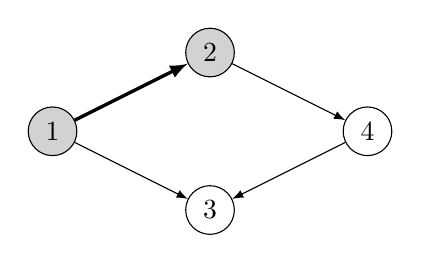
\begin{tikzpicture}
            \node[draw,circle,fill=gray!35] (A)at(0,0) {1};
            \node[draw,circle,fill=gray!35] (B)at(2,1) {2};
            \node[draw,circle] (C)at(2,-1) {3};
            \node[draw,circle] (D)at(4,0) {4};


            \draw[->,>=latex, very thick] (A) -- (B);
            \draw[->,>=latex] (A) -- (C);
            \draw[->,>=latex] (B) -- (D);
            \draw[<-,>=latex] (C) -- (D);
        \end{tikzpicture}
        \captionof{figure}{Parcours récursif}
    \end{center}

\end{frame}
\begin{frame}
    \frametitle{}

    \begin{center}
        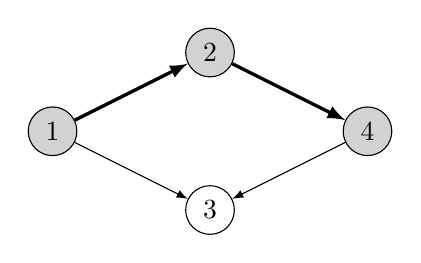
\begin{tikzpicture}
            \node[draw,circle,fill=gray!35] (A)at(0,0) {1};
            \node[draw,circle,fill=gray!35] (B)at(2,1) {2};
            \node[draw,circle] (C)at(2,-1) {3};
            \node[draw,circle,fill=gray!35] (D)at(4,0) {4};


            \draw[->,>=latex, very thick] (A) -- (B);
            \draw[->,>=latex] (A) -- (C);
            \draw[->,>=latex, very thick] (B) -- (D);
            \draw[<-,>=latex] (C) -- (D);
        \end{tikzpicture}
        \captionof{figure}{Parcours récursif}
    \end{center}

\end{frame}
\begin{frame}
    \frametitle{}

    \begin{center}
        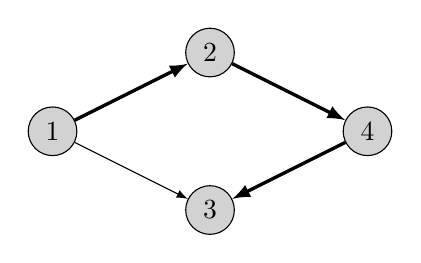
\begin{tikzpicture}
            \node[draw,circle,fill=gray!35] (A)at(0,0) {1};
            \node[draw,circle,fill=gray!35] (B)at(2,1) {2};
            \node[draw,circle,fill=gray!35] (C)at(2,-1) {3};
            \node[draw,circle,fill=gray!35] (D)at(4,0) {4};


            \draw[->,>=latex, very thick] (A) -- (B);
            \draw[->,>=latex] (A) -- (C);
            \draw[->,>=latex, very thick] (B) -- (D);
            \draw[<-,>=latex, very thick] (C) -- (D);
        \end{tikzpicture}
        \captionof{figure}{Parcours récursif}
    \end{center}

\end{frame}
\begin{frame}
    \frametitle{}

    \begin{center}
        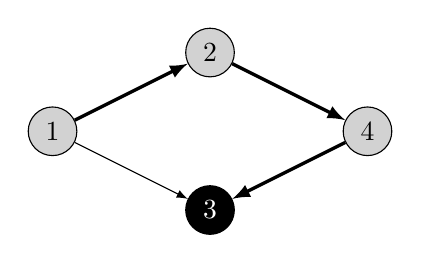
\begin{tikzpicture}
            \node[draw,circle,fill=gray!35] (A)at(0,0) {1};
            \node[draw,circle,fill=gray!35] (B)at(2,1) {2};
            \node[draw,circle,fill=black,text=white] (C)at(2,-1) {3};
            \node[draw,circle,fill=gray!35] (D)at(4,0) {4};


            \draw[->,>=latex, very thick] (A) -- (B);
            \draw[->,>=latex] (A) -- (C);
            \draw[->,>=latex, very thick] (B) -- (D);
            \draw[<-,>=latex, very thick] (C) -- (D);
        \end{tikzpicture}
        \captionof{figure}{Fin du parcours pour \textbf{\texttt{3}}}
    \end{center}

\end{frame}
\begin{frame}
    \frametitle{}

    \begin{center}
        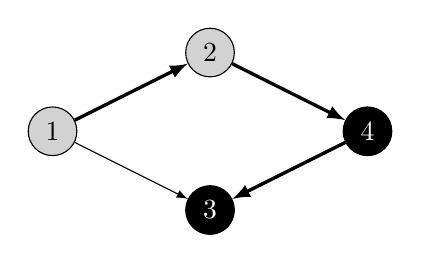
\begin{tikzpicture}
            \node[draw,circle,fill=gray!35] (A)at(0,0) {1};
            \node[draw,circle,fill=gray!35] (B)at(2,1) {2};
            \node[draw,circle,fill=black,text=white] (C)at(2,-1) {3};
            \node[draw,circle,fill=black,text=white] (D)at(4,0) {4};


            \draw[->,>=latex, very thick] (A) -- (B);
            \draw[->,>=latex] (A) -- (C);
            \draw[->,>=latex, very thick] (B) -- (D);
            \draw[<-,>=latex, very thick] (C) -- (D);
        \end{tikzpicture}
        \captionof{figure}{Fin du parcours pour \textbf{\texttt{4}}}
    \end{center}

\end{frame}
\begin{frame}
    \frametitle{}

    \begin{center}
        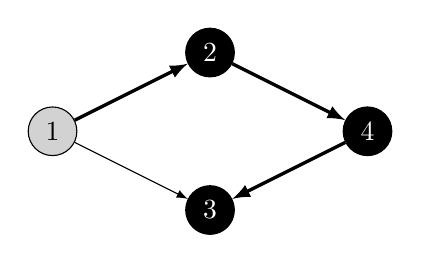
\begin{tikzpicture}
            \node[draw,circle,fill=gray!35] (A)at(0,0) {1};
            \node[draw,circle,fill=black,text=white] (B)at(2,1) {2};
            \node[draw,circle,fill=black,text=white] (C)at(2,-1) {3};
            \node[draw,circle,fill=black,text=white] (D)at(4,0) {4};


            \draw[->,>=latex, very thick] (A) -- (B);
            \draw[->,>=latex] (A) -- (C);
            \draw[->,>=latex, very thick] (B) -- (D);
            \draw[<-,>=latex, very thick] (C) -- (D);
        \end{tikzpicture}
        \captionof{figure}{Fin du parcours pour \textbf{\texttt{2}}}
    \end{center}

\end{frame}
\begin{frame}
    \frametitle{}

    \begin{center}
        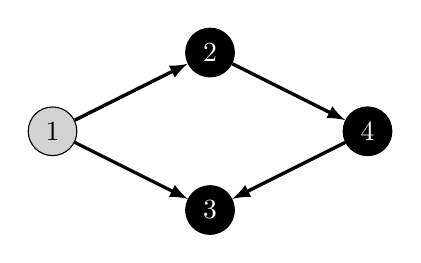
\begin{tikzpicture}
            \node[draw,circle,fill=gray!35] (A)at(0,0) {1};
            \node[draw,circle,fill=black,text=white] (B)at(2,1) {2};
            \node[draw,circle,fill=black,text=white] (C)at(2,-1) {3};
            \node[draw,circle,fill=black,text=white] (D)at(4,0) {4};


            \draw[->,>=latex, very thick] (A) -- (B);
            \draw[->,>=latex, very thick] (A) -- (C);
            \draw[->,>=latex, very thick] (B) -- (D);
            \draw[<-,>=latex, very thick] (C) -- (D);
        \end{tikzpicture}
        \captionof{figure}{\textbf{\texttt{3}} est \textbf{\texttt{NOIR}}: pas de cycle.}
    \end{center}
\end{frame}

\begin{frame}
    \frametitle{}

    \begin{center}
        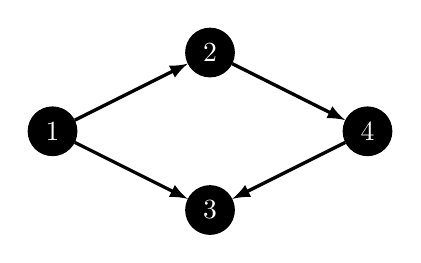
\begin{tikzpicture}
            \node[draw,circle,fill=black,text=white] (A)at(0,0) {1};
            \node[draw,circle,fill=black,text=white] (B)at(2,1) {2};
            \node[draw,circle,fill=black,text=white] (C)at(2,-1) {3};
            \node[draw,circle,fill=black,text=white] (D)at(4,0) {4};


            \draw[->,>=latex, very thick] (A) -- (B);
            \draw[->,>=latex, very thick] (A) -- (C);
            \draw[->,>=latex, very thick] (B) -- (D);
            \draw[<-,>=latex, very thick] (C) -- (D);
        \end{tikzpicture}
        \captionof{figure}{Fin du parcours pour \textbf{\texttt{1}}}
    \end{center}
    \begin{center}
        {\Large Pas de cycle}
    \end{center}
\end{frame}
%autre cas
\begin{frame}
    \frametitle{}

    \begin{center}
        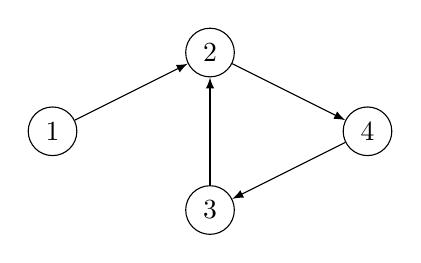
\begin{tikzpicture}
            \node[draw,circle] (A)at(0,0) {1};
            \node[draw,circle] (B)at(2,1) {2};
            \node[draw,circle] (C)at(2,-1) {3};
            \node[draw,circle] (D)at(4,0) {4};
            \draw[->,>=latex] (A) -- (B);
            \draw[<-,>=latex] (B) -- (C);
            \draw[->,>=latex] (B) -- (D);
            \draw[<-,>=latex] (C) -- (D);
        \end{tikzpicture}
        \captionof{figure}{Initialisation}
    \end{center}
\end{frame}
\begin{frame}
    \frametitle{}

    \begin{center}
        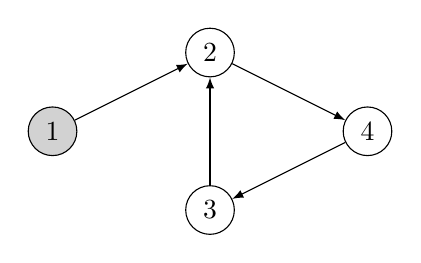
\begin{tikzpicture}
            \node[draw,circle,fill=gray!35] (A)at(0,0) {1};
            \node[draw,circle] (B)at(2,1) {2};
            \node[draw,circle] (C)at(2,-1) {3};
            \node[draw,circle] (D)at(4,0) {4};
            \draw[->,>=latex] (A) -- (B);
            \draw[<-,>=latex] (B) -- (C);
            \draw[->,>=latex] (B) -- (D);
            \draw[<-,>=latex] (C) -- (D);
        \end{tikzpicture}
        \captionof{figure}{Début du parcours}
    \end{center}
\end{frame}
\begin{frame}
    \frametitle{}

    \begin{center}
        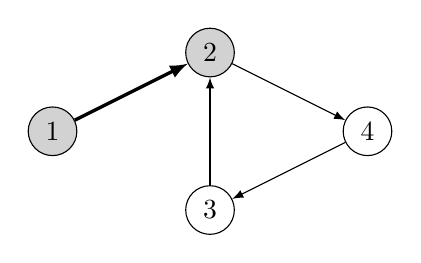
\begin{tikzpicture}
            \node[draw,circle,fill=gray!35] (A)at(0,0) {1};
            \node[draw,circle,fill=gray!35] (B)at(2,1) {2};
            \node[draw,circle] (C)at(2,-1) {3};
            \node[draw,circle] (D)at(4,0) {4};
            \draw[->,>=latex, very thick] (A) -- (B);
            \draw[<-,>=latex] (B) -- (C);
            \draw[->,>=latex] (B) -- (D);
            \draw[<-,>=latex] (C) -- (D);
        \end{tikzpicture}
        \captionof{figure}{Parcours récursif}
    \end{center}
\end{frame}
\begin{frame}
    \frametitle{}

    \begin{center}
        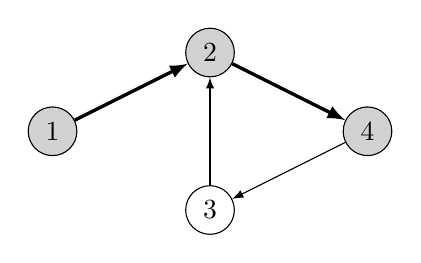
\begin{tikzpicture}
            \node[draw,circle,fill=gray!35] (A)at(0,0) {1};
            \node[draw,circle,fill=gray!35] (B)at(2,1) {2};
            \node[draw,circle] (C)at(2,-1) {3};
            \node[draw,circle,fill=gray!35] (D)at(4,0) {4};
            \draw[->,>=latex, very thick] (A) -- (B);
            \draw[<-,>=latex] (B) -- (C);
            \draw[->,>=latex, very thick] (B) -- (D);
            \draw[<-,>=latex] (C) -- (D);
        \end{tikzpicture}
        \captionof{figure}{Parcours récursif}
    \end{center}
\end{frame}
\begin{frame}
    \frametitle{}

    \begin{center}
        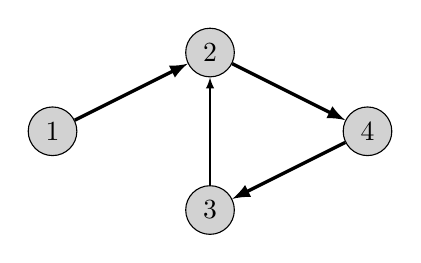
\begin{tikzpicture}
            \node[draw,circle,fill=gray!35] (A)at(0,0) {1};
            \node[draw,circle,fill=gray!35] (B)at(2,1) {2};
            \node[draw,circle,fill=gray!35] (C)at(2,-1) {3};
            \node[draw,circle,fill=gray!35] (D)at(4,0) {4};
            \draw[->,>=latex, very thick] (A) -- (B);
            \draw[<-,>=latex] (B) -- (C);
            \draw[->,>=latex, very thick] (B) -- (D);
            \draw[<-,>=latex, very thick] (C) -- (D);
        \end{tikzpicture}
        \captionof{figure}{Parcours récursif}
    \end{center}
\end{frame}
\begin{frame}
    \frametitle{}

    \begin{center}
        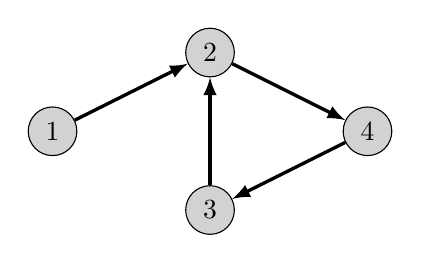
\begin{tikzpicture}
            \node[draw,circle,fill=gray!35] (A)at(0,0) {1};
            \node[draw,circle,fill=gray!35] (B)at(2,1) {2};
            \node[draw,circle,fill=gray!35] (C)at(2,-1) {3};
            \node[draw,circle,fill=gray!35] (D)at(4,0) {4};
            \draw[->,>=latex, very thick] (A) -- (B);
            \draw[<-,>=latex, very thick] (B) -- (C);
            \draw[->,>=latex, very thick] (B) -- (D);
            \draw[<-,>=latex, very thick] (C) -- (D);
        \end{tikzpicture}
        \captionof{figure}{Le sommet \textbf{\texttt{2}} est \textbf{\texttt{GRIS}}: il y a un cycle.}
    \end{center}
\end{frame}
\begin{frame}
    \frametitle{}

    \begin{aretenir}[]
    Lors du parcours en profondeur, si on rencontre un sommet identifié comme \emph{en cours de parcours} alors il y a un cycle.
    \end{aretenir}

\end{frame}
\section{Algorithme}
\begin{frame}
    \frametitle{Algorithme}

    \begin{center}
        \begin{framed}
            \begin{itemize}
            \item Initialiser chaque sommet à \textbf{BLANC}.
            \item Pour chaque sommet:
                  \begin{itemize}
                      \item Effectuer un parcours en profondeur.
                      \item Si le parcours est un cycle, renvoyer \textbf{\texttt{Vrai}}.
                  \end{itemize}
            \item Renvoyer \textbf{\texttt{Faux}}
        \end{itemize}
        \end{framed}
        \captionof{code}{Vérifier s'il y a un cycle.}
    \end{center}

\end{frame}
\begin{frame}
    \frametitle{}
    \begin{center}
        \begin{framed}
            \begin{itemize}
                \item Initialiser chaque sommet à \textbf{BLANC}.
                \item Pour chaque sommet:
                      \begin{itemize}
                          \item Effectuer un parcours en profondeur.
                          \item Si le parcours est un cycle, renvoyer \textbf{\texttt{Vrai}}.
                      \end{itemize}
                \item Renvoyer \textbf{\texttt{Faux}}
            \end{itemize}
        \end{framed}
        
    \begin{framed}
        \begin{itemize}
            \item Si le sommet est \textbf{\texttt{GRIS}} renvoyer \textbf{\texttt{Vrai}}.
            \item Si le sommet est \textbf{\texttt{NOIR}} renvoyer \textbf{\texttt{Faux}}.
            \item Marquer le sommet \textbf{\texttt{GRIS}}.
            \item pour tous les sommets voisins:
            \begin{itemize}
                \item Effectuer récursivement un parcours en profondeur.
                \item Si le parcours est un cycle, renvoyer \textbf{\texttt{Vrai}}.
            \end{itemize}
            \item Marquer le sommet \textbf{\texttt{NOIR}}.
            \item Renvoyer \textbf{\texttt{Faux}}.
        \end{itemize}
    \end{framed}
    \captionof{code}{Effectuer un parcours en profondeur.}
\end{center}

\end{frame}
\subsection{Implémentation}
\begin{frame}
    \frametitle{Implémentation}
    \begin{center}
        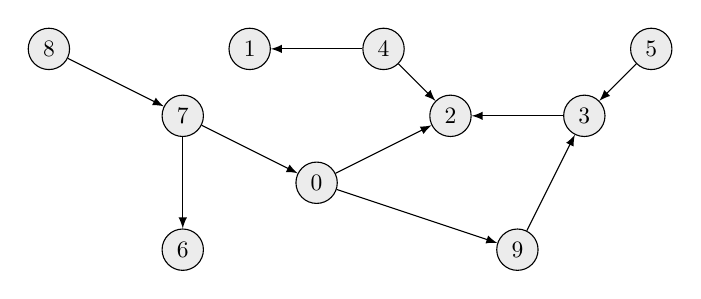
\begin{tikzpicture}[scale=0.85, transform shape]
            \node[draw,circle,fill=gray!15] (A)at(0,0) {0};
            \node[draw,circle,fill=gray!15] (B)at(-1,2) {1};
            \node[draw,circle,fill=gray!15] (C)at(2,1) {2};
            \node[draw,circle,fill=gray!15] (D)at(4,1) {3};
            \node[draw,circle,fill=gray!15] (E)at(1,2) {4};
            \node[draw,circle,fill=gray!15] (F)at(5,2) {5};
            \node[draw,circle,fill=gray!15] (G)at(-2,-1) {6};
            \node[draw,circle,fill=gray!15] (H)at(-2,1) {7};
            \node[draw,circle,fill=gray!15] (I)at(-4,2) {8};
            \node[draw,circle,fill=gray!15] (J)at(3,-1) {9};
            \draw[->,>=latex] (E) -- (B);
            \draw[->,>=latex] (A) -- (C);
            \draw[<-,>=latex] (A) -- (H);
            \draw[->,>=latex] (A) -- (J);
            \draw[<-,>=latex] (H) -- (I);
            \draw[->,>=latex] (H) -- (G);
            \draw[<-,>=latex] (C) -- (E);
            \draw[<-,>=latex] (C) -- (D);
            %\draw[-,>=latex] (C) -- (J);
            \draw[<-,>=latex] (D) -- (J);
            \draw[<-,>=latex] (D) -- (F);
        \end{tikzpicture}
    \end{center}
    \begin{activite}
    \begin{enumerate}
        \item Reprendre le graphe du TP précédent.
        \item Écrire la fonction \textbf{\texttt{a\_cycle(mat: list) $\rightarrow$ bool}} qui lance un parcours depuis chaque sommet.
        \item Écrire la fonction récursive \textbf{\texttt{dfs(mat: list, dep: int, vis: list) $\rightarrow$ bool}} qui effectue le parcours en profondeur.
    \end{enumerate}
    \end{activite}

\end{frame}
\begin{frame}[fragile]
    \frametitle{Correction}

\begin{center}
\begin{lstlisting}[language=Python , basicstyle=\ttfamily\small, xleftmargin=0.2em, xrightmargin=0em]
BLANC, GRIS, NOIR = 0, 1, 2

def a_cycle(mat: list) -> bool:
    visites = [BLANC for _ in range(len(mat))]
    for i in range(len(mat)):
        # lance un parcours depuis chaque sommet
        if dfs(mat, i, visites):
            return True
    return False
\end{lstlisting}
\end{center}  

\end{frame}
\begin{frame}[fragile]
    \frametitle{Correction}

\begin{center}
\begin{lstlisting}[language=Python , basicstyle=\ttfamily\small, xleftmargin=0.2em, xrightmargin=0em]
def dfs(mat: list, dep: int, vis: list) -> bool:
    if vis[dep] == GRIS:  # cycle
        return True
    if vis[dep] == NOIR:
        return False

    # marque le sommet en cours de visite
    vis[dep] = GRIS
    for i in range(len(mat[dep])):
        # c'est un successeur
        if mat[dep][i] == 1:
            if dfs(mat, i, vis):
                # remontée des appels récursifs
                return True

    # fin de la visite
    vis[dep] = NOIR
    return False
\end{lstlisting}
\end{center}  

\end{frame}
\begin{frame}
    \frametitle{}
    \begin{center}
        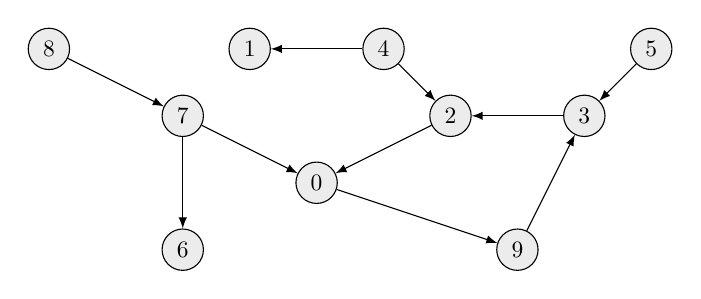
\begin{tikzpicture}[scale=0.85, transform shape]
            \node[draw,circle,fill=gray!15] (A)at(0,0) {0};
            \node[draw,circle,fill=gray!15] (B)at(-1,2) {1};
            \node[draw,circle,fill=gray!15] (C)at(2,1) {2};
            \node[draw,circle,fill=gray!15] (D)at(4,1) {3};
            \node[draw,circle,fill=gray!15] (E)at(1,2) {4};
            \node[draw,circle,fill=gray!15] (F)at(5,2) {5};
            \node[draw,circle,fill=gray!15] (G)at(-2,-1) {6};
            \node[draw,circle,fill=gray!15] (H)at(-2,1) {7};
            \node[draw,circle,fill=gray!15] (I)at(-4,2) {8};
            \node[draw,circle,fill=gray!15] (J)at(3,-1) {9};
            \draw[->,>=latex] (E) -- (B);
            \draw[<-,>=latex] (A) -- (C);
            \draw[<-,>=latex] (A) -- (H);
            \draw[->,>=latex] (A) -- (J);
            \draw[<-,>=latex] (H) -- (I);
            \draw[->,>=latex] (H) -- (G);
            \draw[<-,>=latex] (C) -- (E);
            \draw[<-,>=latex] (C) -- (D);
            %\draw[-,>=latex] (C) -- (J);
            \draw[<-,>=latex] (D) -- (J);
            \draw[<-,>=latex] (D) -- (F);
        \end{tikzpicture}
    \end{center}
    \begin{activite}
    Modifier la matrice pour créer un cycle et tester la fonction à nouveau.
    \end{activite}

\end{frame}
\begin{frame}[fragile]
    \frametitle{Correction}

\begin{center}
\begin{lstlisting}[language=Python , basicstyle=\ttfamily\small, xleftmargin=2em, xrightmargin=2em]
cycle_oui = [
    [0, 0, 0, 0, 0, 0, 0, 0, 0, 1],
    [0, 0, 0, 0, 0, 0, 0, 0, 0, 0],
    [1, 0, 0, 0, 0, 0, 0, 0, 0, 0],
    [0, 0, 1, 0, 0, 0, 0, 0, 0, 0],
    [0, 1, 1, 0, 0, 0, 0, 0, 0, 0],
    [0, 0, 0, 1, 0, 0, 0, 0, 0, 0],
    [0, 0, 0, 0, 0, 0, 0, 0, 0, 0],
    [1, 0, 0, 0, 0, 0, 1, 0, 0, 0],
    [0, 0, 0, 0, 0, 0, 0, 1, 0, 0],
    [0, 0, 0, 1, 0, 0, 0, 0, 0, 0]]

print(a_cycle(cycle_oui))
\end{lstlisting}
\end{center}

\end{frame}
\end{document}